\documentclass[]{article}

\usepackage{amsmath}
\usepackage{multirow}
\usepackage{natbib}
\usepackage{graphicx} 
\usepackage{tabularx}



\begin{document}

\title{A Two-Stage Classification Pipeline for Discovering Thermodynamically Stable and Mechanically Robust ABO3 Perovskites}

\author{Denario}
\date{Anthropic, Gemini \& OpenAI servers. Planet Earth.}

\maketitle
\begin{abstract}
High-throughput discovery of novel ABO$_3$ perovskites is frequently impeded by computational datasets containing sparse and physically unreliable elastic properties. To overcome this challenge, we introduce a two-stage classification pipeline that circumvents direct regression on noisy data by sequentially filtering for thermodynamic stability and mechanical viability. First, a gradient boosting classifier, trained on a dataset of 1283 compounds, predicts thermodynamic stability, employing a rigorous Leave-One-Cluster-Out cross-validation to ensure the model generalizes across diverse chemical families. Second, instead of regressing on flawed elastic moduli, a dedicated classifier trained on a physically-filtered subset of materials distinguishes mechanically viable structures from unstable or unphysical ones with high fidelity. We integrate these models into a multi-objective optimization framework to screen 1068 uncharacterized materials, explicitly penalizing candidates with high predictive uncertainty derived from Gaussian Process Regression to ensure reliability. This integrated approach successfully identifies a Pareto front of 16 promising candidates that optimally balance stability and mechanical robustness. Our methodology shortlists novel materials, including DyVO$_3$ and YCrO$_3$, for targeted computational and experimental validation, demonstrating that a classification-first strategy is a powerful tool for navigating imperfect materials data.
\end{abstract}








\section{Introduction}
\label{sec:intro}
The ABO$_3$ perovskite crystal structure represents a cornerstone of modern materials science, offering a vast compositional landscape for discovering materials with functional properties critical for applications in photovoltaics, catalysis, and electronics. High-throughput computational screening, driven by first-principles calculations, is an essential tool for navigating this expansive chemical space, accelerating the discovery cycle from theoretical prediction to experimental synthesis. However, the efficacy of this data-driven paradigm is fundamentally limited by the quality and completeness of the underlying computational data.

A significant bottleneck in high-throughput workflows arises from the challenge of reliably computing mechanical properties. While thermodynamic stability, often quantified by the energy above the convex hull ($E_{hull}$), is a robust and well-established metric, calculated elastic properties are frequently sparse and plagued by physically unrealistic artifacts. Datasets often contain entries with negative bulk ($K$) or shear ($G$) moduli, which signify structural instabilities that can arise from numerical convergence issues or from performing calculations on dynamically unstable phases. Attempting to train standard regression models on such flawed data is a critical flaw; these models are easily biased by extreme outliers and unphysical values, leading to poor generalization and unreliable predictions for novel materials.

To overcome this challenge, we introduce a two-stage classification pipeline that circumvents the pitfalls of direct regression on noisy elastic data. Our approach reframes the problem by prioritizing qualitative assessment over quantitative prediction for identifying mechanically robust materials. The first stage of our pipeline employs a classifier to predict thermodynamic stability, ensuring that only compounds likely to be synthesizable are passed forward for further consideration. The second, and central, stage addresses mechanical robustness. Instead of attempting to predict the exact values of elastic moduli, a dedicated classifier distinguishes between mechanically viable and unstable structures. This model is trained exclusively on a physically-vetted subset of data, allowing it to learn the structural and chemical features associated with mechanical integrity without being corrupted by the nonsensical data points that undermine regression-based approaches.

We integrate these sequential classifiers into a multi-objective optimization framework to screen a large space of uncharacterized ABO$_3$ compounds, seeking candidates that simultaneously satisfy the criteria for both thermodynamic stability and mechanical robustness. To further enhance the reliability of our screening, we explicitly incorporate model uncertainty derived from a Gaussian Process Regression model, penalizing candidates for which predictions are not confident. This integrated strategy allows us to efficiently map the trade-offs between competing material properties and isolate a Pareto front of novel, high-confidence perovskite candidates. Our work demonstrates that a classification-first strategy provides a powerful and robust framework for materials discovery, particularly when navigating the imperfect and often unreliable datasets characteristic of high-throughput computational science.

\section{Methods}
\label{sec:methods}
\subsection{Dataset and feature engineering}
The foundation of this study is a dataset comprising 1283 unique ABO$_3$ perovskite compounds sourced from a high-throughput computational materials database. For each compound, we utilized a set of structural and chemical features derived from its stoichiometry and relaxed crystal structure. Key descriptors included the Goldschmidt tolerance factor ($\tau$) and the octahedral factor ($\mu$), which quantify the geometric compatibility of the constituent ions within the perovskite lattice. To capture the effects of structural strain, we engineered features representing the deviation from ideal geometries, namely $\tau_{strain} = |\tau - 1.0|$ and $\mu_{strain} = |\mu - 0.57|$. Additional features included elemental properties such as ionic radii and electronegativity differences, as well as macroscopic properties like density and formation energy per atom. The crystal volume was log-transformed to mitigate the influence of its skewed distribution. Finally, the space group number of each compound was used to classify it into one of the 23 Glazer tilt systems, providing a categorical representation of the octahedral tilting patterns.

The target properties for our models were thermodynamic stability, mechanical properties, and electronic band gap. Thermodynamic stability was treated as a binary classification label, where a material with an energy above the convex hull ($E_{hull}$) of 0 eV/atom was labeled as stable. Mechanical properties were represented by the Voigt-Reuss-Hill (VRH) averages of the bulk ($K_{VRH}$) and shear ($G_{VRH}$) moduli. The electronic band gap was used as a continuous target variable.

\subsection{Thermodynamic stability model}
To predict thermodynamic stability, we trained a Gradient Boosting Classifier (GBC). The classification task was framed to distinguish stable compounds ($E_{hull} = 0$ eV/atom) from metastable ones ($E_{hull} > 0$ eV/atom). Given the significant class imbalance in the dataset, where only 13.1\% of the compounds are stable, model evaluation was performed using the Area Under the Precision-Recall Curve (AUC-PR), which is more informative than accuracy or ROC-AUC for imbalanced problems.

To ensure the model's ability to generalize to new chemical families, we employed a rigorous Leave-One-Cluster-Out (LOCO) cross-validation strategy. In this scheme, the data was partitioned into 53 clusters, each containing all compounds with the same A-site element. During each fold of the cross-validation, the model was trained on 52 clusters and validated on the single held-out cluster, thereby testing its performance on entirely unseen chemical compositions.

\subsection{Mechanical property models}
The raw dataset for mechanical properties was both sparse, with elastic constants available for only 16.8\% of the compounds, and contaminated with unphysical values such as negative or extremely large moduli. To address this, we first applied a physical filter, creating a training subset of 207 materials that satisfied the criteria $0 < K_{VRH} < 300$ GPa and $G_{VRH} > 0$.

Our primary approach to mechanical robustness was to reframe the problem from regression to classification. A Mechanical Viability Classifier, also a GBC model, was trained on the full 215-sample subset to distinguish the 207 physically consistent compounds from the unphysical or unstable ones. This model provides a direct probabilistic score of a material's mechanical viability. Its performance was assessed using 5-fold stratified cross-validation, with metrics including accuracy, F1 score, precision, and recall.

To quantify the uncertainty of predictions for uncharacterized materials, we also trained a Gaussian Process Regressor (GPR) on the 207-sample filtered subset to predict $K_{VRH}$ and $G_{VRH}$. The GPR employed a composite kernel consisting of a Constant kernel multiplied by a Mat\'{e}rn kernel with $\nu=1.5$, summed with a WhiteKernel to account for noise. The primary output from the GPR used in our subsequent analysis was the predictive variance, $\sigma^2$, which serves as a measure of the model's confidence for any given prediction.

\subsection{Electronic property model}
The distribution of the electronic band gap is bimodal, with 48.6\% of the materials being metals (band gap = 0 eV). To accurately model this zero-inflated distribution, we implemented a two-stage Hurdle model.
\begin{enumerate}
    \item \textbf{Metallicity Classifier:} A GBC was trained to solve a binary classification problem: predicting whether a material is a metal (`is\_metal` = True) or not.
    \item \textbf{Band Gap Regressor:} A Gradient Boosting Regressor (GBR) was trained exclusively on the subset of non-metallic compounds. The target variable for this model was the log-transformed band gap, $\log(1 + \text{band\_gap})$, to handle the right-skewed distribution of non-zero values.
\end{enumerate}
The final band gap prediction for a given material was determined by first applying the classifier. If the material was predicted to be a metal, its band gap was set to 0 eV. Otherwise, the regressor was used to predict the log-transformed band gap, which was then converted back to the original scale. The performance of the integrated Hurdle model was evaluated using the Mean Absolute Error (MAE) on a held-out test set.

\subsection{Multi-objective optimization for candidate screening}
We developed a multi-objective optimization framework to screen the 1068 uncharacterized compounds in our dataset. The goal was to identify novel candidates that simultaneously exhibit high thermodynamic stability and high mechanical robustness, while also ensuring the reliability of the predictions. The two primary objectives for maximization were:
\begin{enumerate}
    \item The predicted probability of thermodynamic stability from the LOCO-validated GBC.
    \item The predicted probability of mechanical viability from the dedicated viability classifier.
\end{enumerate}
To explicitly account for model uncertainty, we introduced a penalty term derived from the GPR models. The mechanical viability score was adjusted by a penalty proportional to the model's predictive uncertainty. The penalized viability score for a candidate material $i$ was calculated as:
\begin{equation}
    S_{penalized}(i) = P_{viability}(i) \times \left(1 - \frac{\bar{\sigma}^2(i) - \min(\bar{\sigma}^2)}{\max(\bar{\sigma}^2) - \min(\bar{\sigma}^2)}\right)
\end{equation}
where $P_{viability}(i)$ is the raw probability from the viability classifier and $\bar{\sigma}^2(i)$ is the average predictive variance from the GPR models for $K_{VRH}$ and $G_{VRH}$ for that material. This formulation penalizes candidates for which the model has low confidence, steering the search towards more reliable regions of the chemical space. By plotting the candidates in the space defined by stability probability and penalized viability, we identified a Pareto front of optimal materials representing the best trade-offs between the competing objectives.

\section{Results}
\label{sec:results}
\subsection{Thermodynamic stability classification}

The first stage of our pipeline addresses the prediction of thermodynamic stability, a binary classification task where stable compounds are defined as having an energy above the convex hull of 0 eV/atom. Given the significant class imbalance in our dataset, with only 13.1\% of the 1283 compounds being stable, we employed a Gradient Boosting Classifier (GBC) evaluated with a rigorous Leave-One-Cluster-Out (LOCO) cross-validation. By partitioning the data into 53 clusters based on the A-site element, this strategy ensures the model is tested on its ability to generalize to entirely new chemical families, preventing overly optimistic performance estimates that can arise from random data splits.

The model achieved an Area Under the Precision-Recall Curve (AUC-PR) of 0.353 and an F1-score of 0.320. As illustrated in Figure \ref{fig:image0}, the precision-recall curve demonstrates that the model's performance is substantially better than the no-skill baseline of 0.131 (the positive class frequency). This indicates a strong capability to enrich a pool of candidates with thermodynamically stable materials, which is the primary goal of this initial filtering stage. The chemical heterogeneity of the dataset, where stability rates vary drastically between A-site groups, underscores the necessity of the LOCO approach for building a truly generalizable model that learns the underlying physical principles of stability rather than memorizing compositional patterns.

\begin{figure}[h!]
    \centering
    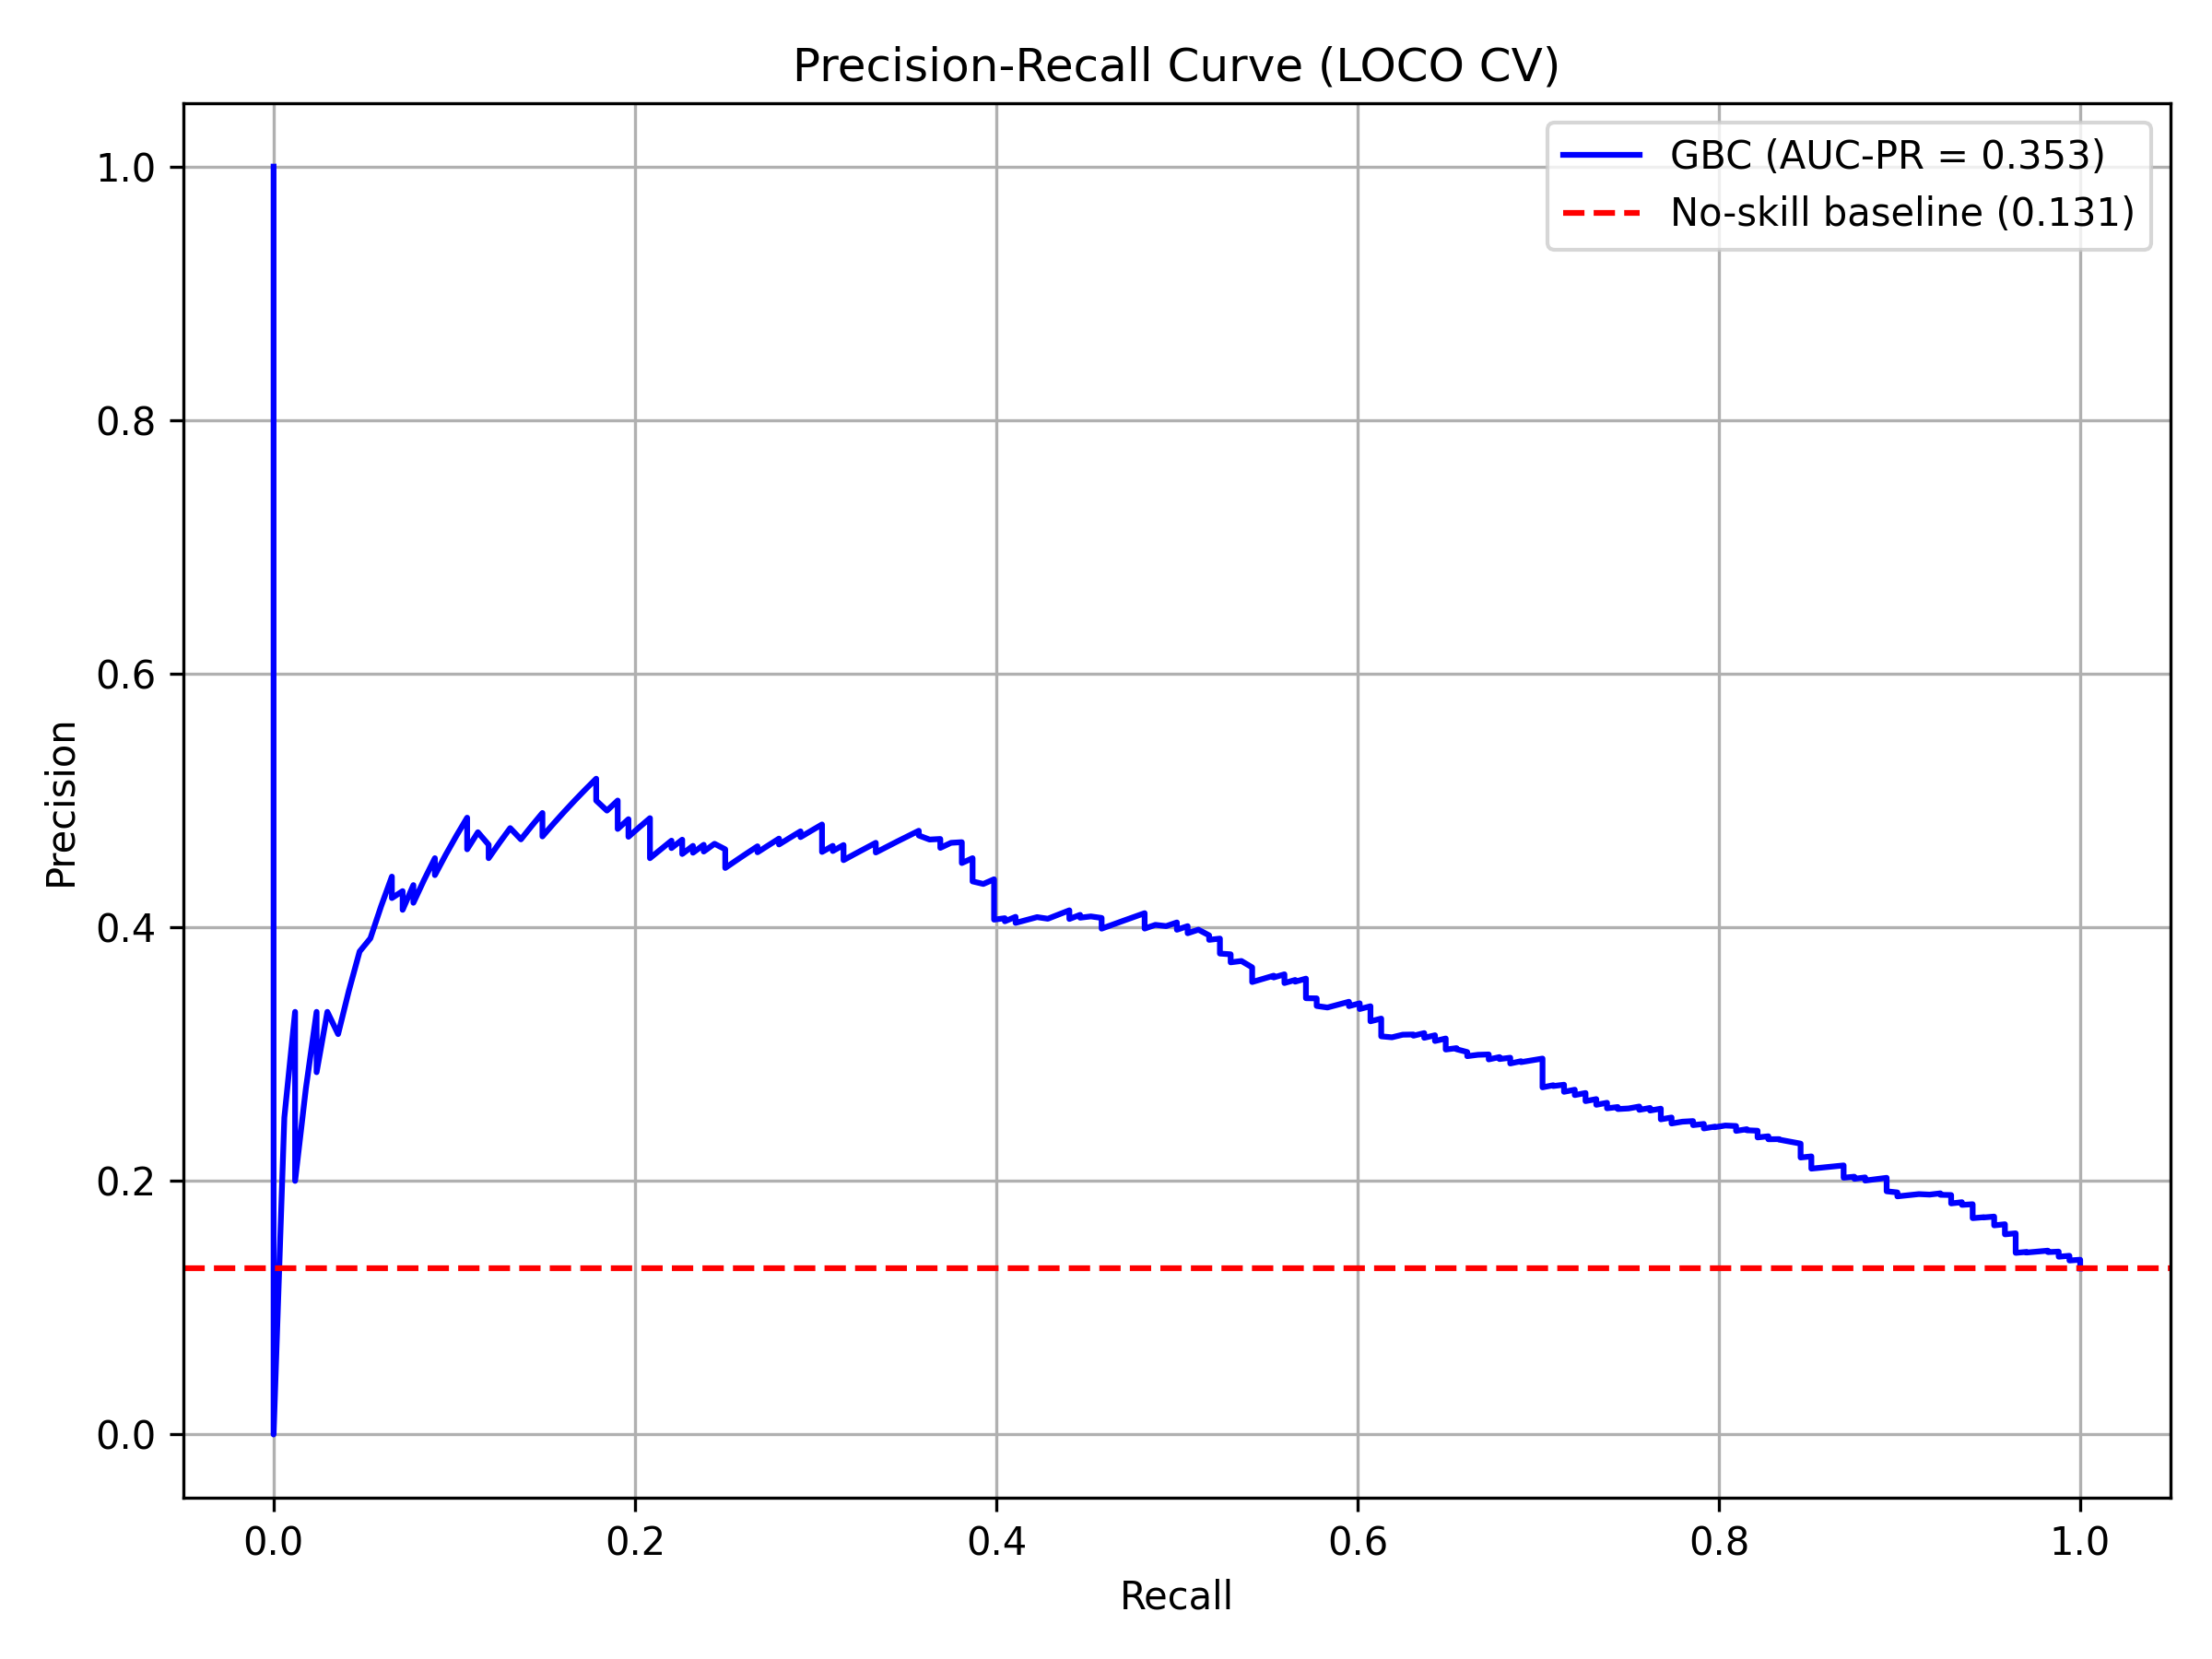
\includegraphics[width=0.5\textwidth]{../input_files/plots/step_2_pr_curve_stability_1_1776245452.png}
    \caption{Precision-Recall curve for the Gradient Boosting Classifier (GBC) predicting the thermodynamic stability of ABO$_3$ perovskites. The model was evaluated using a rigorous Leave-One-Cluster-Out (LOCO) cross-validation strategy, grouped by the A-site element. The resulting Area Under the Curve (AUC-PR) of 0.353 demonstrates a substantial performance improvement over the no-skill baseline of 0.131, which corresponds to the 13.1\% frequency of stable compounds in the dataset. This illustrates the model's ability to effectively enrich a candidate pool with thermodynamically stable materials far beyond random selection.}
    \label{fig:image0}
\end{figure}

\subsection{Mechanical viability classification and uncertainty quantification}

A central challenge in high-throughput materials screening is the prevalence of sparse and unreliable data for mechanical properties. Our dataset reflects this issue, with elastic constants available for only 16.8\% of compounds and numerous entries containing unphysical values (e.g., negative or extremely large moduli) indicative of calculation failures. To circumvent the pitfalls of regressing on this flawed data, we reframed the problem as a binary classification task.

A Mechanical Viability Classifier (a GBC model) was trained to distinguish physically consistent materials (207 samples with $0 < K_{VRH} < 300$ GPa and $G_{VRH} > 0$) from the 8 unphysical or unstable ones. Evaluated with 5-fold stratified cross-validation, this classifier demonstrated exceptional performance in identifying sound candidates, achieving an accuracy of $0.9628 \pm 0.0315$, an F1-score of $0.9805 \pm 0.0170$, and a precision of $0.9762 \pm 0.0147$. This high precision is critical for a screening workflow, as it minimizes the risk of passing mechanically unstable materials to subsequent stages.

In parallel, to quantify the model's confidence when making predictions on uncharacterized materials, we trained Gaussian Process Regressor (GPR) models on the filtered 207-sample subset. While their predictive accuracy for $K_{VRH}$ and $G_{VRH}$ was moderate ($R^2$ scores of 0.7431 and 0.7066, respectively), their primary purpose was to provide a predictive variance, $\sigma^2$. This variance serves as a robust measure of epistemic uncertainty, which we leverage in the final optimization stage to penalize predictions in sparsely populated regions of the chemical space, thereby ensuring the reliability of our discovered candidates.

\subsection{Hurdle model for electronic properties}

The electronic band gap distribution in our dataset is bimodal, with 48.6\% of materials being metals (band gap = 0 eV). Standard regression models struggle with such zero-inflated data. To address this, we implemented a two-stage Hurdle model. The first stage, a GBC classifier, predicts whether a material is a metal. On a held-out test set, this classifier achieved an accuracy of 0.7938 and a ROC-AUC of 0.8848, effectively separating the two classes.

The second stage, a Gradient Boosting Regressor, was trained exclusively on the non-metallic compounds to predict their log-transformed band gaps. The integrated Hurdle model first uses the classifier; if a material is predicted to be a metal, its band gap is set to 0 eV. Otherwise, the regressor's prediction is used. This combined approach achieved a Mean Absolute Error (MAE) of 0.5225 eV across the entire test set. The parity plot in Figure \ref{fig:image1} visually confirms the model's performance, showing a high concentration of correct predictions at 0 eV for metals and a strong correlation for non-metals. While this model accurately reproduces the DFT-PBE values, it is important to note that these are known to systematically underestimate experimental band gaps.

\begin{figure}[h!]
    \centering
    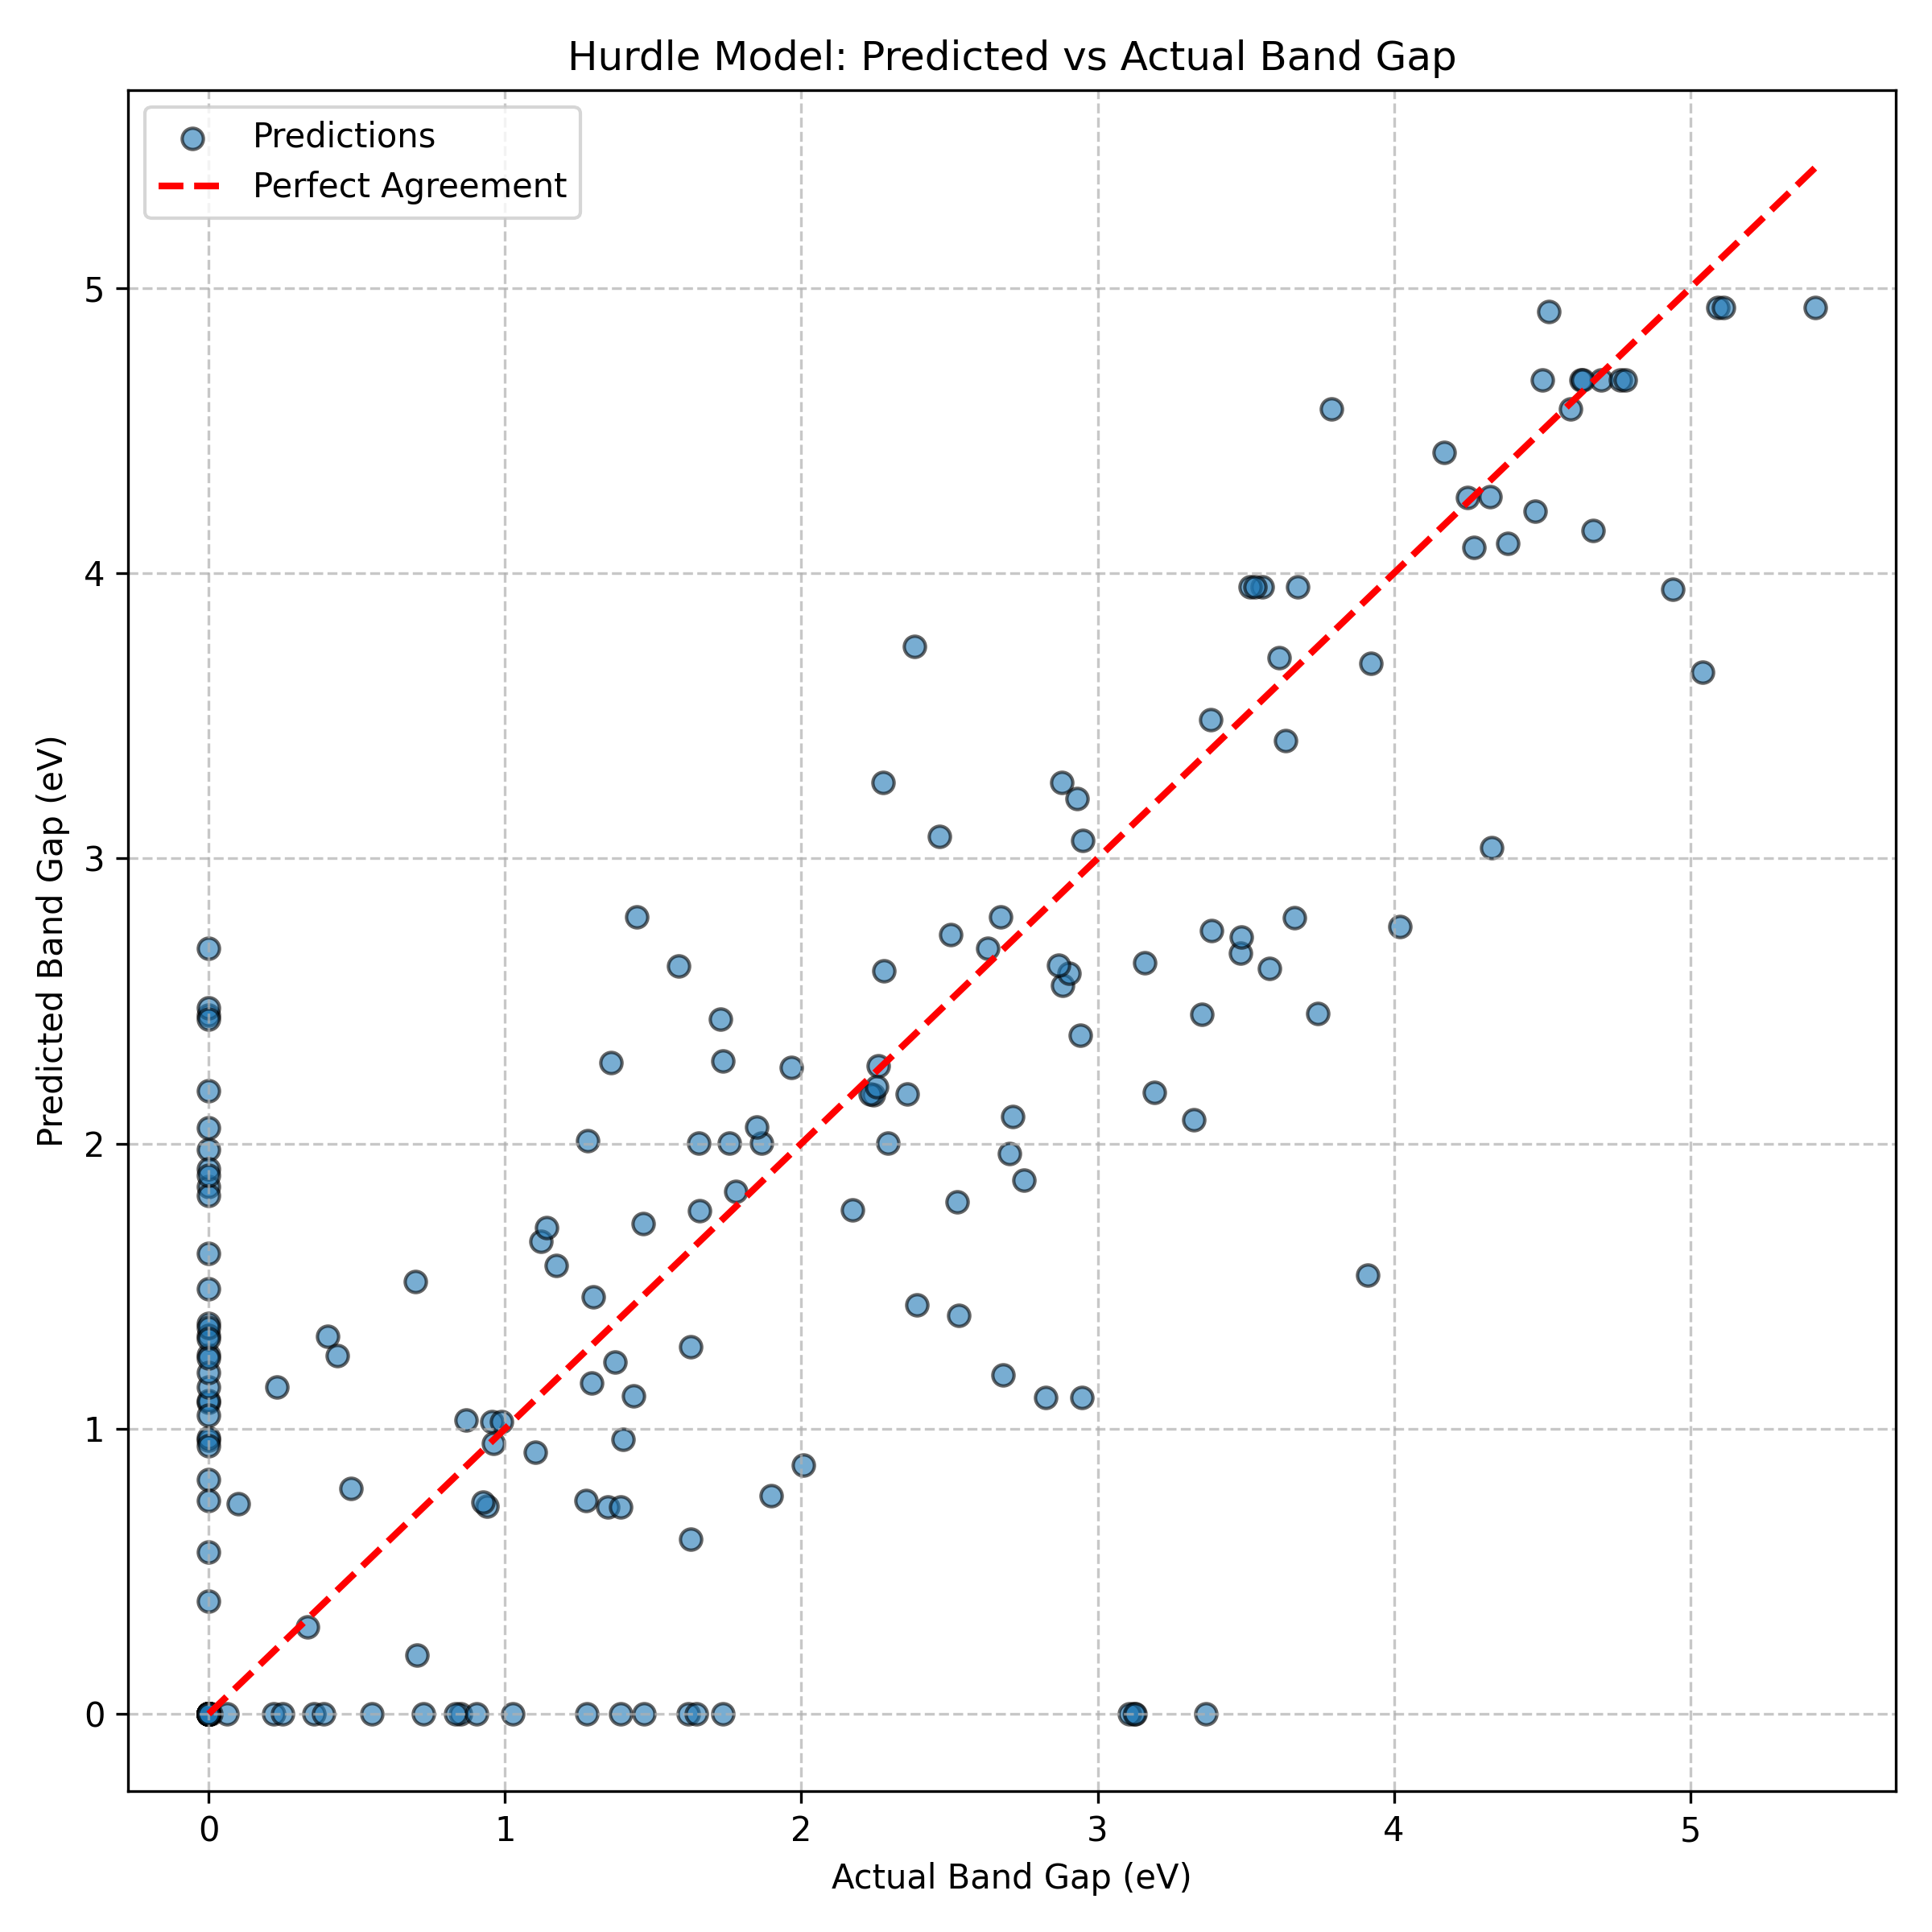
\includegraphics[width=0.5\textwidth]{../input_files/plots/step_4_parity_plot_bandgap_1_1776245655.png}
    \caption{Performance of the two-stage Hurdle model for electronic band gap prediction on the held-out test set. This parity plot compares the model's predicted band gap against the actual DFT-PBE values. The model's ability to handle the bimodal, zero-inflated nature of the data is evident, with a high concentration of predictions correctly identifying metallic materials (actual band gap = 0 eV). For non-metallic compounds, the predictions are scattered around the line of perfect agreement (red dashed line), and the integrated model achieves a Mean Absolute Error of 0.5225 eV across the entire test set.}
    \label{fig:image1}
\end{figure}

\subsection{Model interpretability and physical drivers}

To ensure our models learned physically meaningful relationships, we used SHapley Additive exPlanations (SHAP) to interpret their predictions.

\subsubsection{Thermodynamic stability}
The SHAP analysis for the stability model, summarized in Figure \ref{fig:image2}, reveals that the most influential features are rooted in crystallographic and chemical principles. The Goldschmidt tolerance factor strain ($\tau_{strain} = |\tau - 1.0|$) and octahedral factor strain ($\mu_{strain} = |\mu - 0.57|$) are paramount. Low values for these strain metrics, corresponding to geometries close to the ideal perovskite structure, strongly drive the model to predict stability (high positive SHAP values). This confirms the model has learned the well-established principle that minimizing lattice strain is crucial for phase stability. Additionally, a moderate-to-high electronegativity difference (`en\_diff`) and the presence of specific high-symmetry Glazer tilt systems (e.g., `a0a0a0`) were also identified as key indicators of stability.

\begin{figure}[h!]
    \centering
    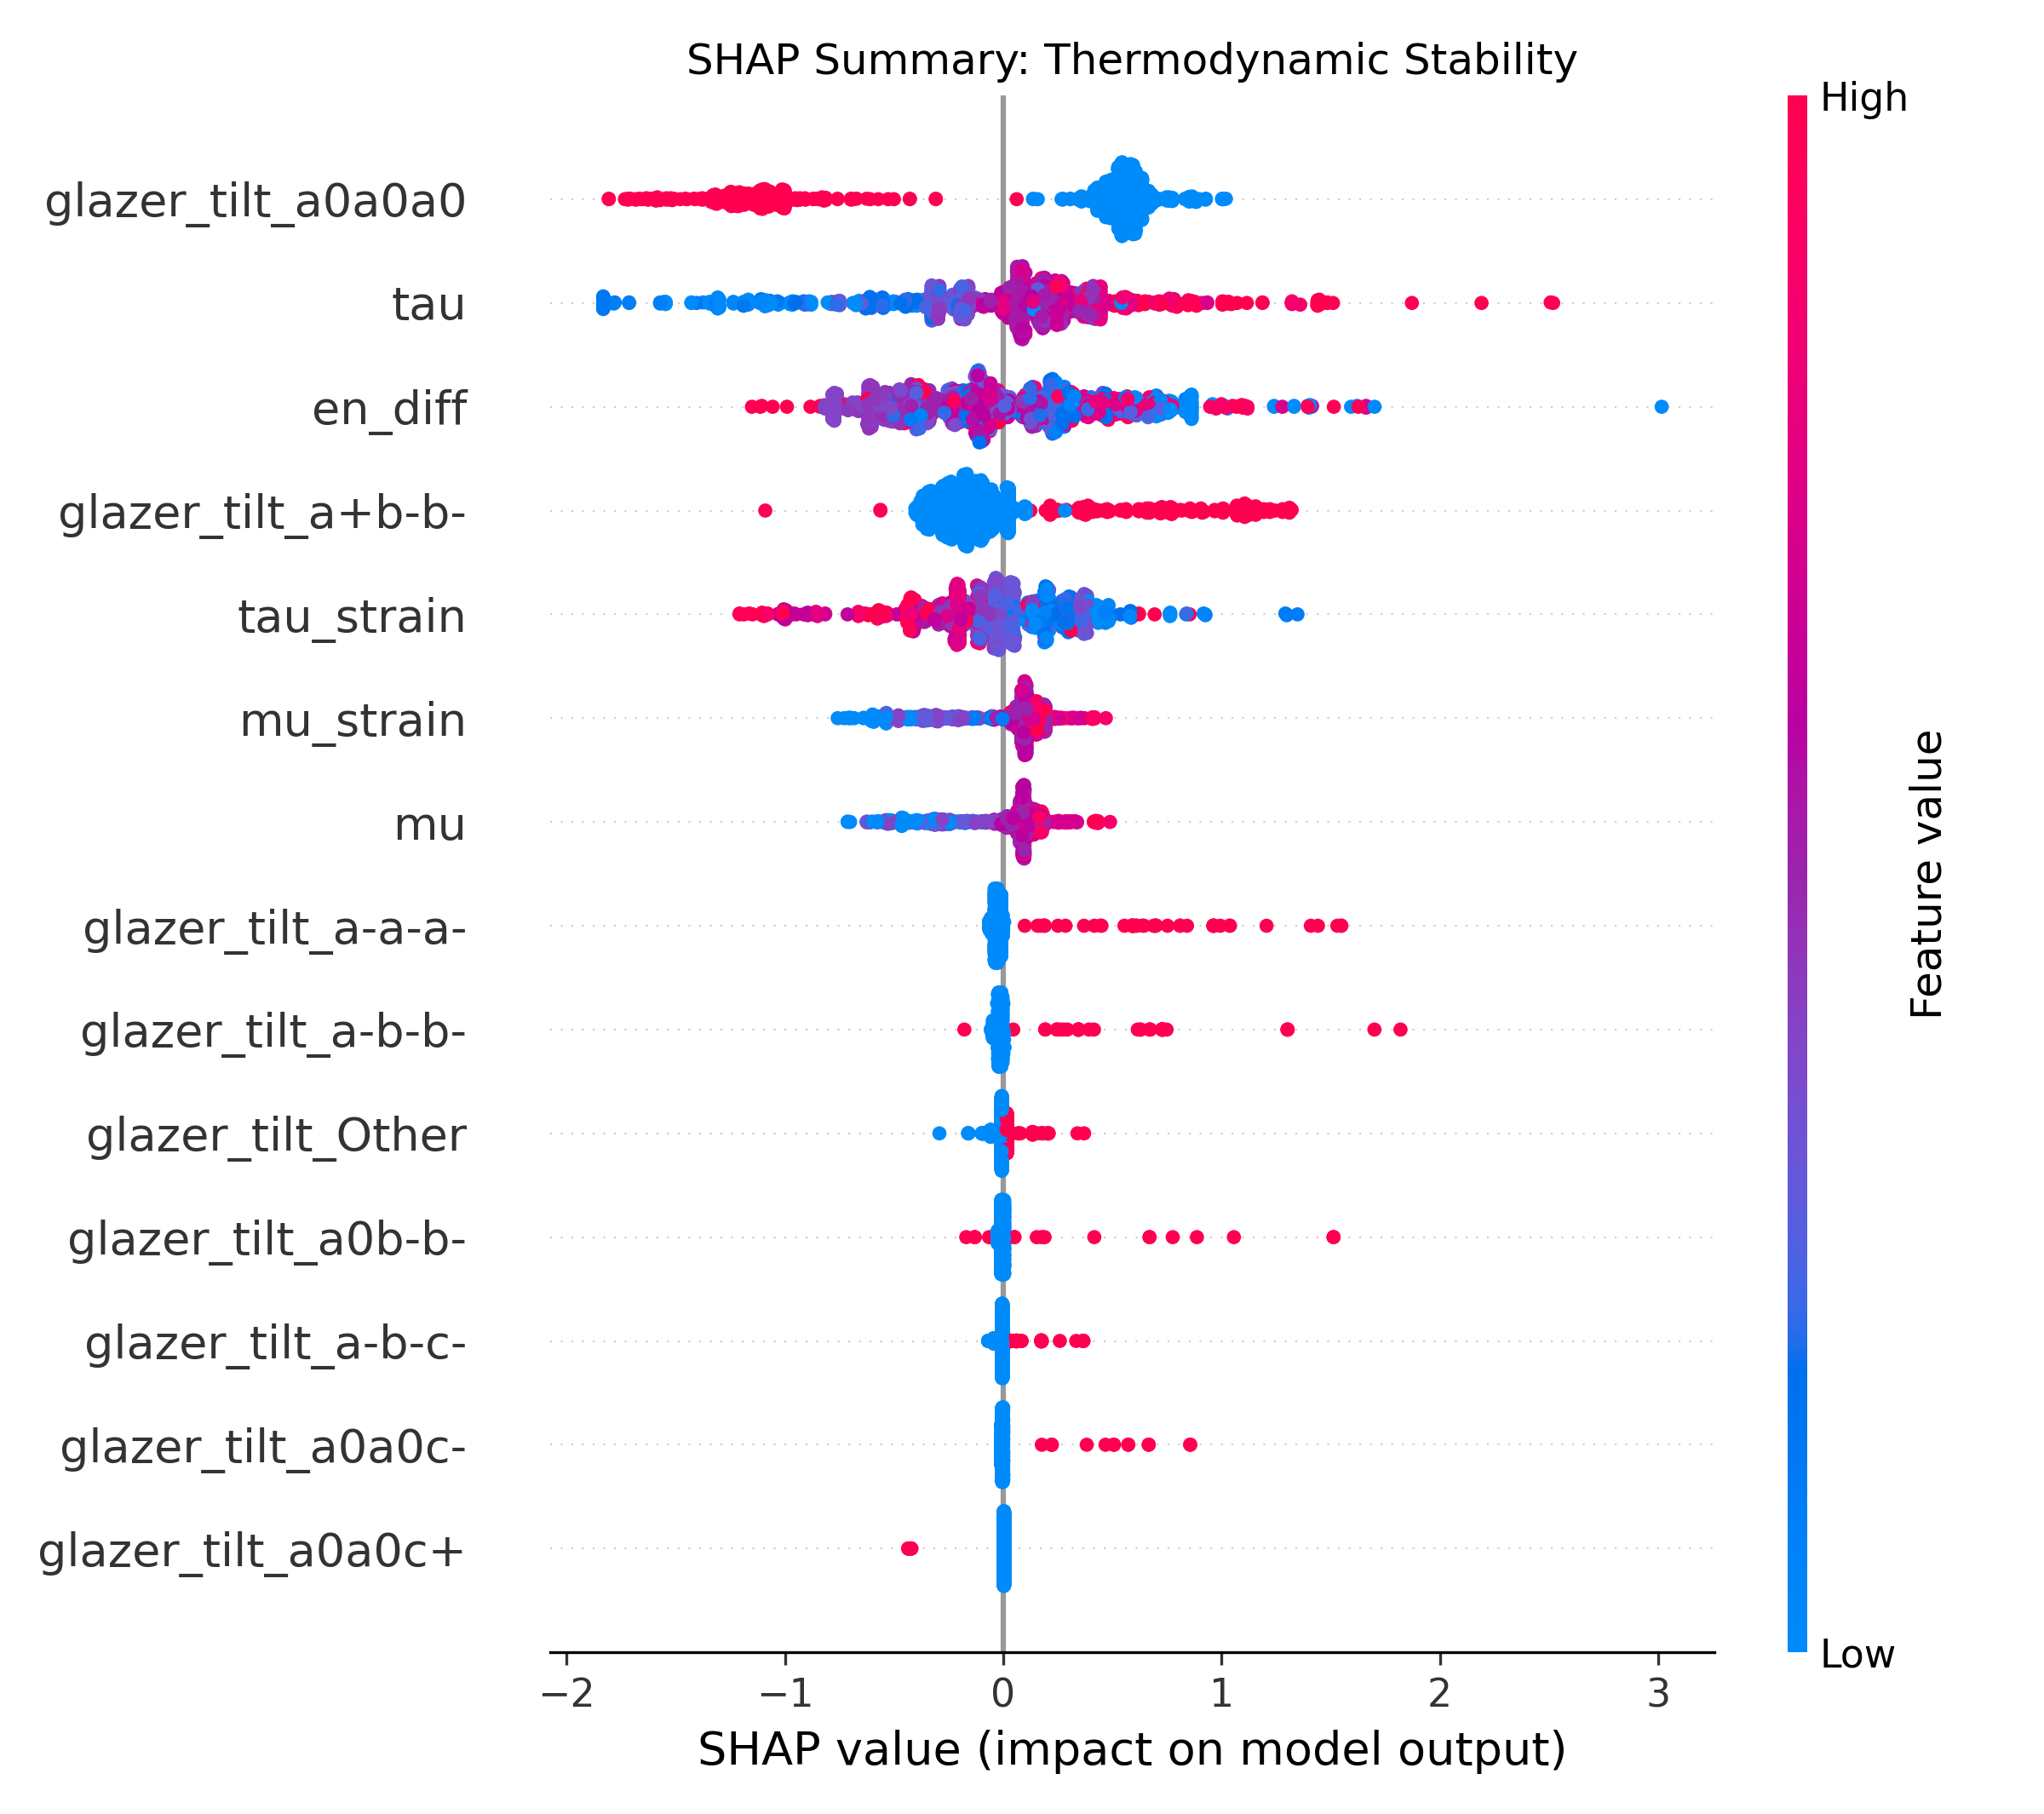
\includegraphics[width=0.5\textwidth]{../input_files/plots/step_6_shap_summary_stability_1_1776245837.png}
    \caption{SHAP summary plot for the thermodynamic stability model, illustrating the impact of the most predictive features. The analysis reveals that low structural strain, indicated by low values for Goldschmidt tolerance factor strain (`tau\_strain`) and octahedral factor strain (`mu\_strain`), strongly increases the predicted probability of stability (positive SHAP values). Similarly, a high electronegativity difference (`en\_diff`) and the presence of specific Glazer tilt systems, such as the high-symmetry cubic `glazer\_tilt\_a0a0a0`, are key drivers favoring thermodynamic stability.}
    \label{fig:image2}
\end{figure}

\subsubsection{Mechanical viability}
The Mechanical Viability Classifier learned a different set of physical rules, as shown in Figure \ref{fig:image3}. The most important features were macroscopic properties: `density`, `formation\_energy\_per\_atom`, and `log\_volume`. High density, a more negative formation energy, and smaller volume are all strong predictors of mechanical viability. This suggests the model identified a key physical correlation: materials that are thermodynamically stable (deep potential energy well) and densely packed are less likely to exhibit the structural instabilities or unphysical configurations that lead to failed elastic constant calculations. The ionic radius of the A-site cation (`A\_radius`) and crystal system also play a role, indicating that specific atomic packing arrangements are inherently more robust.

\begin{figure}[h!]
    \centering
    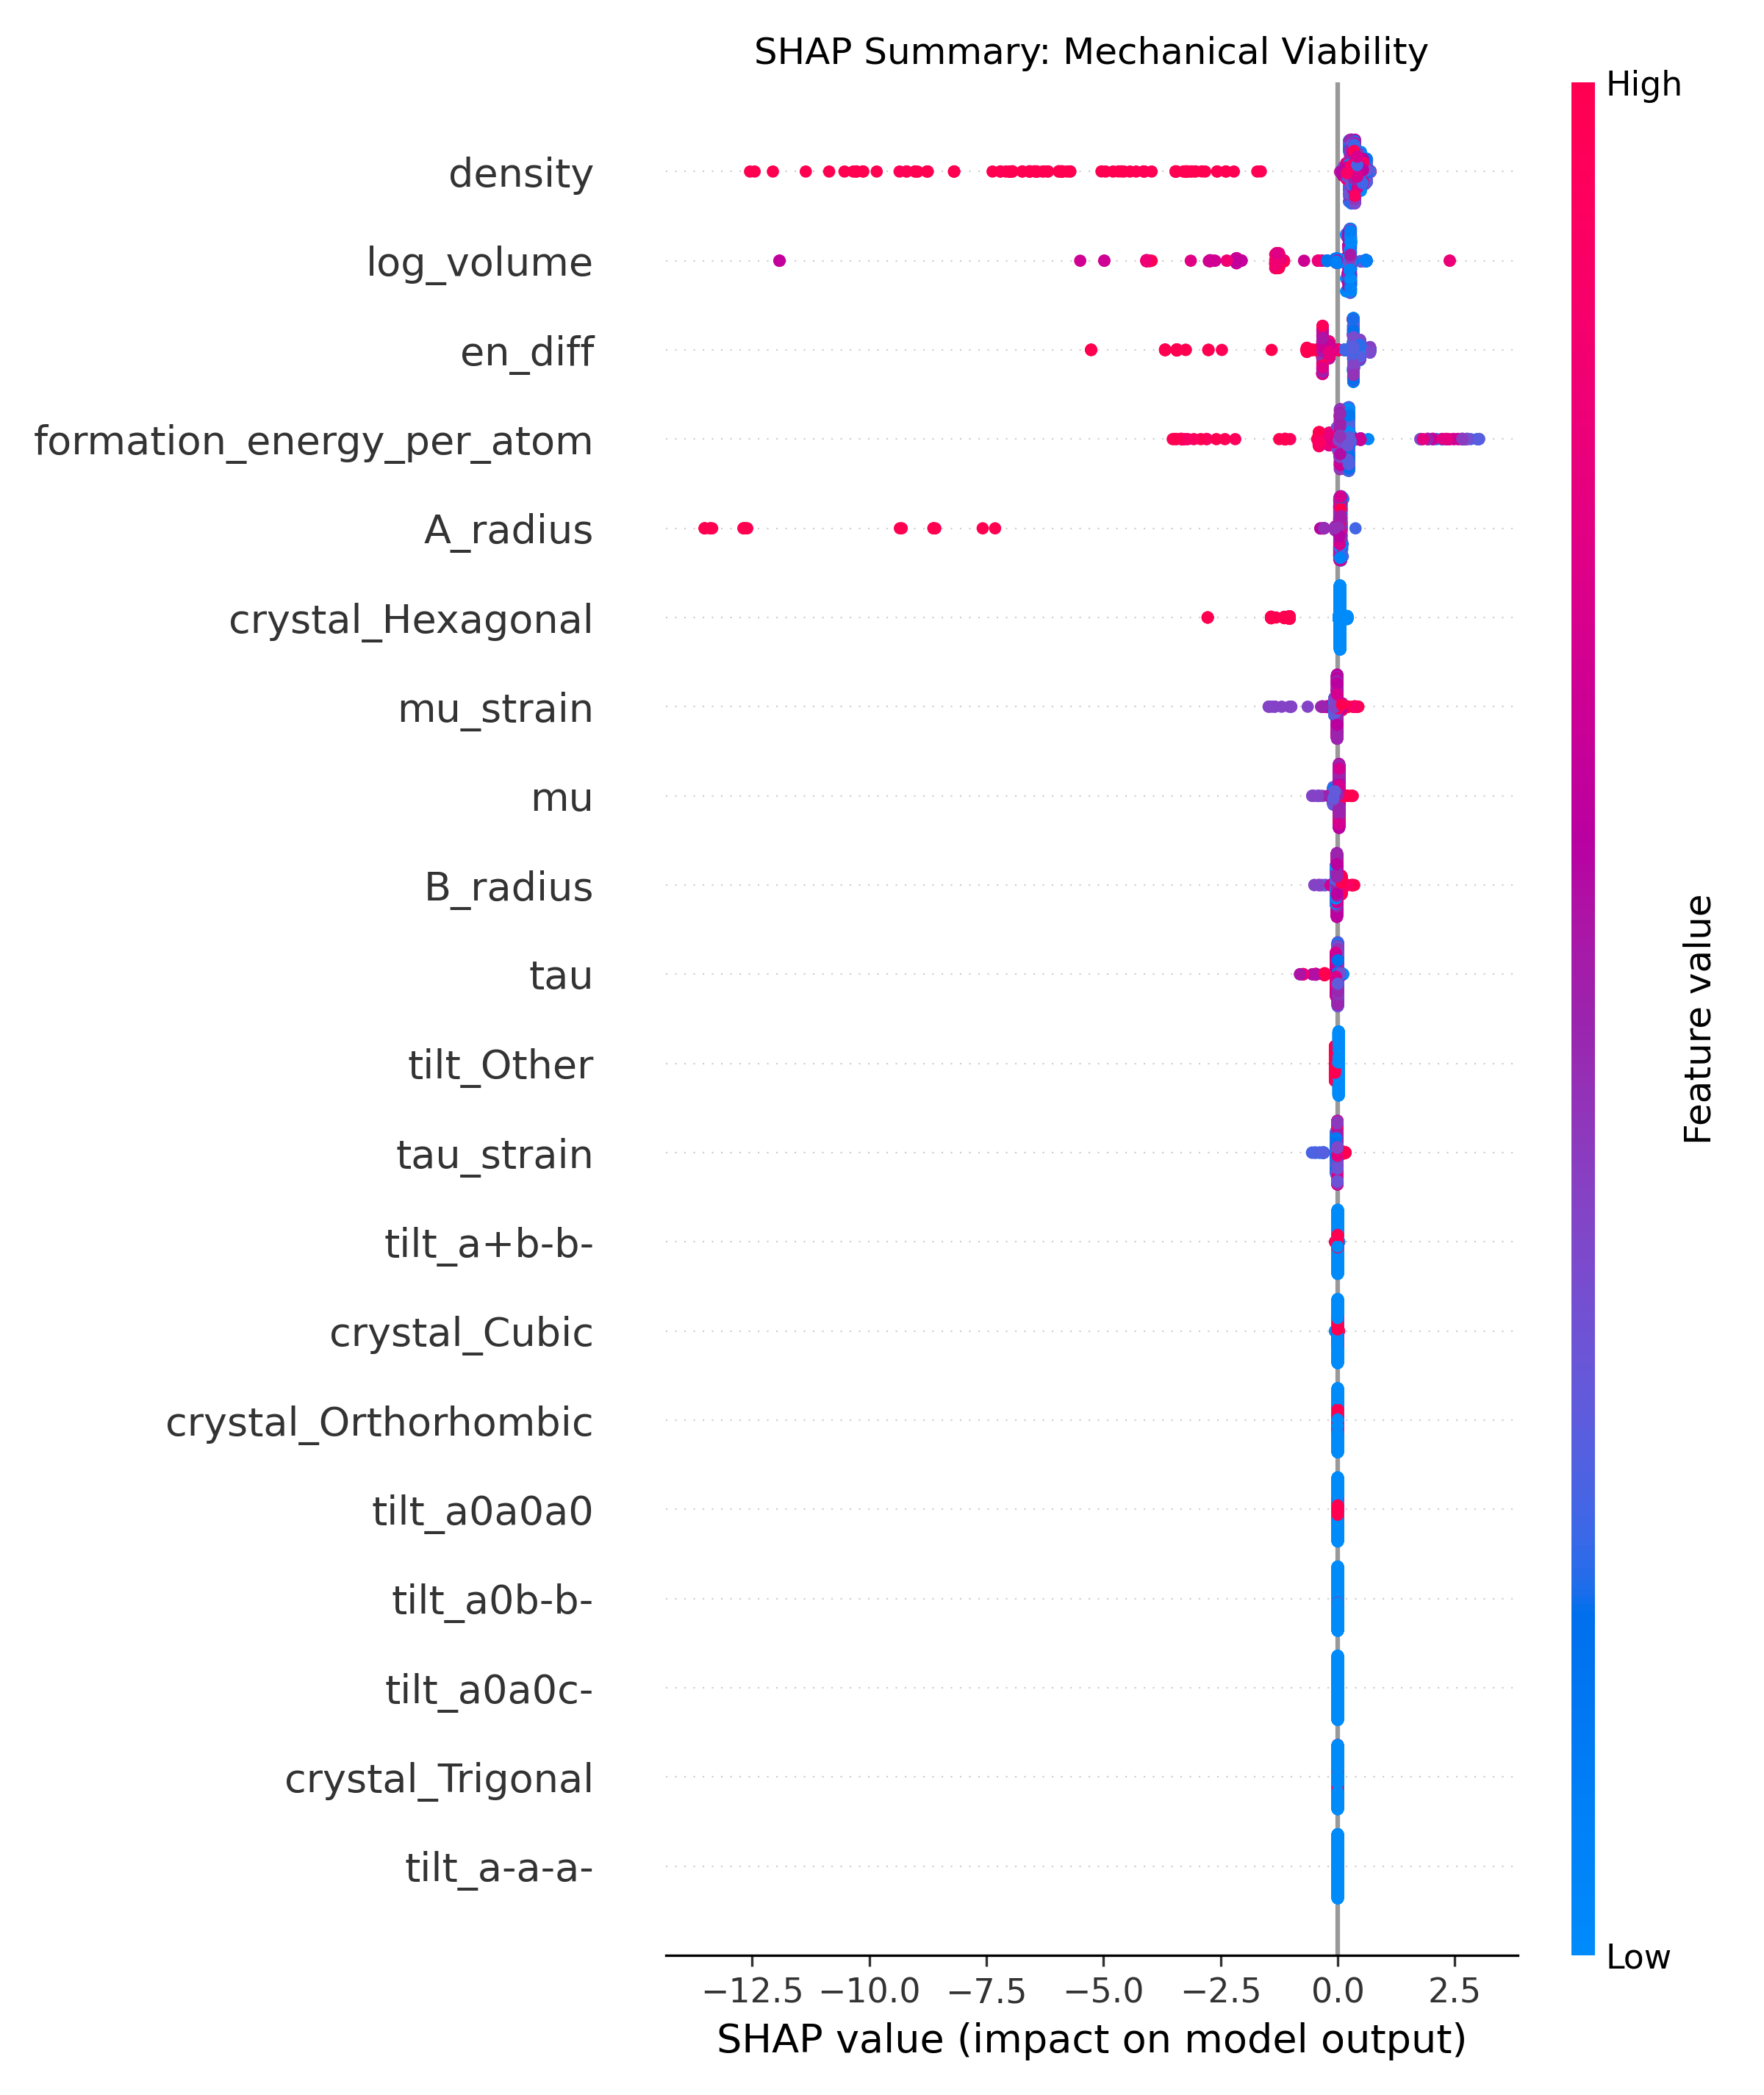
\includegraphics[width=0.5\textwidth]{../input_files/plots/step_6_shap_summary_viability_1_1776245837.png}
    \caption{SHAP summary plot for the Mechanical Viability Classifier, where features are ranked by importance. Each point represents a material, with its color indicating the feature value (red for high, blue for low) and its x-position showing the impact on the prediction of viability. The plot demonstrates that high density, low log\_volume, and a more negative formation\_energy\_per\_atom are the strongest predictors of mechanical viability. The A-site ionic radius (A\_radius) and the presence of a hexagonal crystal structure (crystal\_Hexagonal) are also identified as significant contributing factors.}
    \label{fig:image3}
\end{figure}

\subsection{Multi-objective screening and candidate identification}

The final step of our workflow was to screen 1068 uncharacterized compounds to identify novel candidates that are both thermodynamically stable and mechanically robust. We performed a multi-objective optimization, maximizing two objectives: the probability of thermodynamic stability and a penalized probability of mechanical viability. The viability score was penalized using the predictive variance from the GPR models, as defined in the Methods section, to explicitly disfavor candidates for which the model's predictions are highly uncertain.

Plotting the candidates in this two-dimensional objective space, as shown in Figure \ref{fig:image4}, reveals a distinct Pareto front of 16 optimal materials. These candidates represent the best possible trade-offs between stability and reliable mechanical robustness. The effect of the uncertainty penalty is evident, as it suppresses candidates that might otherwise have a high raw viability score but are located in regions of chemical space where the model lacks confidence.

\begin{figure}[h!]
    \centering
    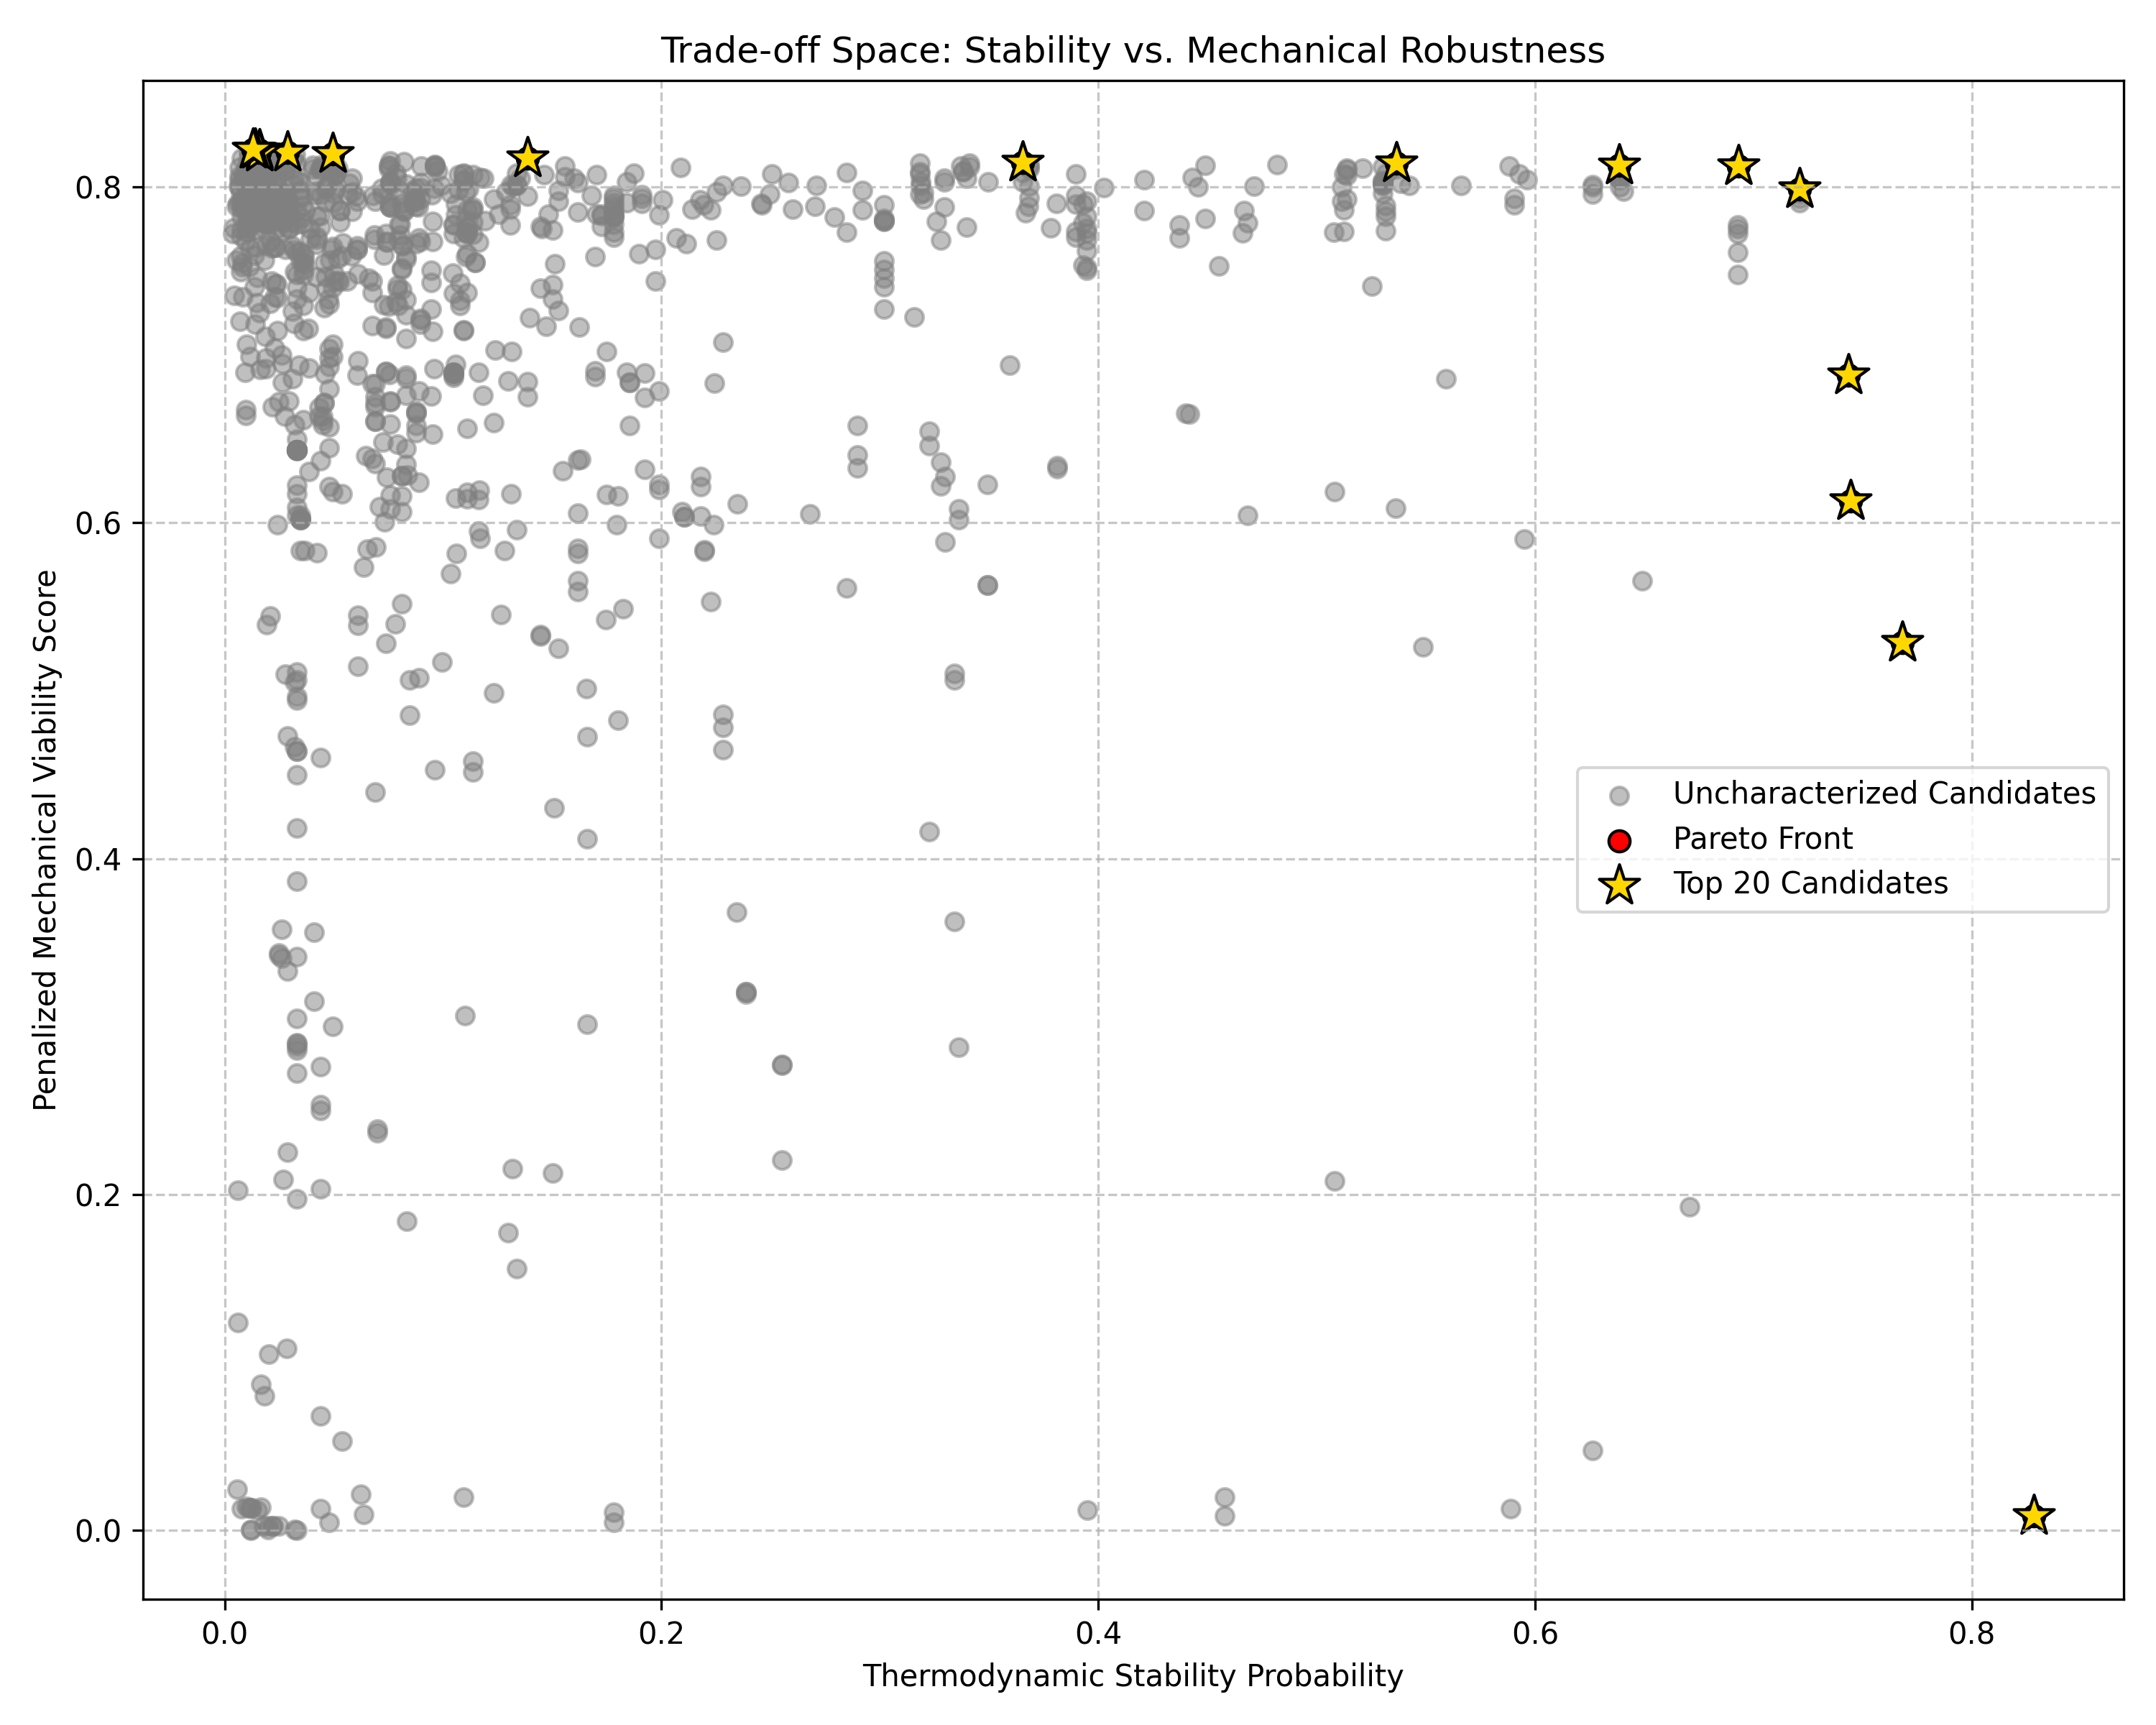
\includegraphics[width=0.5\textwidth]{../input_files/plots/step_6_tradeoff_space_1_1776245837.png}
    \caption{Multi-objective optimization trade-off space for 1068 uncharacterized ABO$_3$ perovskite candidates, plotting the predicted thermodynamic stability probability against the mechanical viability score. The viability score is penalized by the predictive uncertainty derived from Gaussian Process Regressor models for the elastic moduli, thereby down-weighting candidates in regions of high model uncertainty. The plot reveals a distinct Pareto front, with the top 20 optimal candidates highlighted (yellow stars), which represent the best compromises between high stability and high, low-uncertainty mechanical robustness.}
    \label{fig:image4}
\end{figure}

The top 5 candidates from the Pareto front are detailed in Table \ref{tab:candidates}. These materials, led by DyVO$_3$ and YCrO$_3$, are predicted to have a high likelihood of both stability and mechanical viability with low associated uncertainty. The identified candidates are predominantly rare-earth vanadates, chromates, and rhodates, along with a few alkaline-earth silicates. These chemical families appear to possess the optimal combination of ionic radii, cohesive energy, and dense packing that our models identified as being critical for both thermodynamic and mechanical integrity. This shortlist provides a set of high-confidence targets for subsequent first-principles validation and experimental synthesis.

\begin{table*}[t]
\centering
\caption{Top 5 Pareto-optimal perovskite candidates identified through multi-objective screening. Candidates are ranked by the sum of their predicted thermodynamic stability probability and penalized mechanical viability score. The unpenalized viability probability and the GPR-derived uncertainty penalty are also listed to illustrate the effect of the penalty term.}
\label{tab:candidates}
\begin{tabular}{lccccc}
\hline
\hline
Rank & Compound (ID) & Stability Prob. & Penalized Viability & Unpenalized Viability Prob. & Uncertainty Penalty \\
\hline
1 & DyVO$_3$ (mp-22789) & 0.721 & 0.799 & 0.9999 & 0.201 \\
2 & YCrO$_3$ (mp-18725) & 0.693 & 0.813 & 0.9999 & 0.187 \\
3 & NdRhO$_3$ (mp-4582) & 0.639 & 0.813 & 0.9999 & 0.187 \\
4 & SrSiO$_3$ (mp-3978) & 0.743 & 0.688 & 0.9999 & 0.312 \\
5 & BaSiO$_3$ (mp-776084) & 0.744 & 0.613 & 0.9999 & 0.387 \\
\hline
\end{tabular}
\end{table*}

\section{Conclusions}
\label{sec:conclusions}
In this work, we addressed a critical bottleneck in the high-throughput computational discovery of ABO$_3$ perovskites: the prevalence of sparse and physically unreliable data for mechanical properties. Standard regression models often fail when trained on such datasets, leading to poor predictions. To overcome this, we developed and validated a two-stage classification pipeline designed to sequentially screen for thermodynamic stability and mechanical robustness.

Our methodology was built upon a dataset of 1283 perovskite compounds. The first stage employed a Gradient Boosting Classifier, validated with a rigorous Leave-One-Cluster-Out cross-validation scheme, to identify thermodynamically stable materials. The second, and central, stage reframed the problem of mechanical property prediction. Instead of regressing on noisy elastic moduli, we trained a dedicated classifier to distinguish mechanically viable structures from unphysical or unstable ones. This classification-first approach avoids the pitfalls of training on flawed data. To ensure the reliability of our screening, we integrated these models into a multi-objective optimization framework that explicitly penalizes candidates with high predictive uncertainty, as quantified by a Gaussian Process Regressor.

Our results demonstrate the efficacy of this strategy. The stability model proved capable of significantly enriching a candidate pool with stable compounds. The mechanical viability classifier achieved high precision, effectively filtering out materials with inconsistent mechanical properties. Interpretability analysis using SHAP confirmed that our models learned physically meaningful principles: thermodynamic stability was primarily driven by low geometric strain, while mechanical viability correlated strongly with high density and negative formation energy. The final multi-objective screening successfully identified a Pareto front of 16 promising candidates that optimally balance stability and mechanical robustness, shortlisting novel materials such as DyVO$_3$ and YCrO$_3$ for further investigation.

We have learned that for materials discovery tasks hampered by imperfect data, a classification-first strategy is a powerful and robust alternative to direct regression. By prioritizing the qualitative identification of viable candidates over the quantitative prediction of flawed target values, our pipeline efficiently navigates a vast chemical space to isolate a small set of high-confidence materials. This work establishes a generalizable framework for accelerating materials discovery in the presence of noisy and incomplete computational datasets.


\bibliography{bibliography}{}
\bibliographystyle{unsrt}

\end{document}
